%!TEX root = ../template.tex
%%%%%%%%%%%%%%%%%%%%%%%%%%%%%%%%%%%%%%%%%%%%%%%%%%%%%%%%%%%%%%%%%%%%
%% chapter3_HardwareDesign.tex
%% NOVA thesis document file
%%
%% Chapter with the Hardware Design part
%%%%%%%%%%%%%%%%%%%%%%%%%%%%%%%%%%%%%%%%%%%%%%%%%%%%%%%%%%%%%%%%%%%%

\typeout{NT FILE chapter3_HardwareDesign.tex}

\chapter{Hardware Design}\label{cha:chapter3_HardwareDesign}

Meter aqui um pequena introdução do que e mostrado neste capitulo e descrição de seccoes

\section{Architecture and Component Selection}\label{31_Architecture}

The system's desired specifications and requirements exposed throughout Section~\ref{sec:II_Specs} allow a redesign of its current architecture (Figure~\ref{fig:architecture_original}), which is presented in Figure~\ref{fig:architecture_new}.

% meter aqui o NOVO diagrama de blocos -- INACABADO;
\begin{figure}[h]
	\centering
	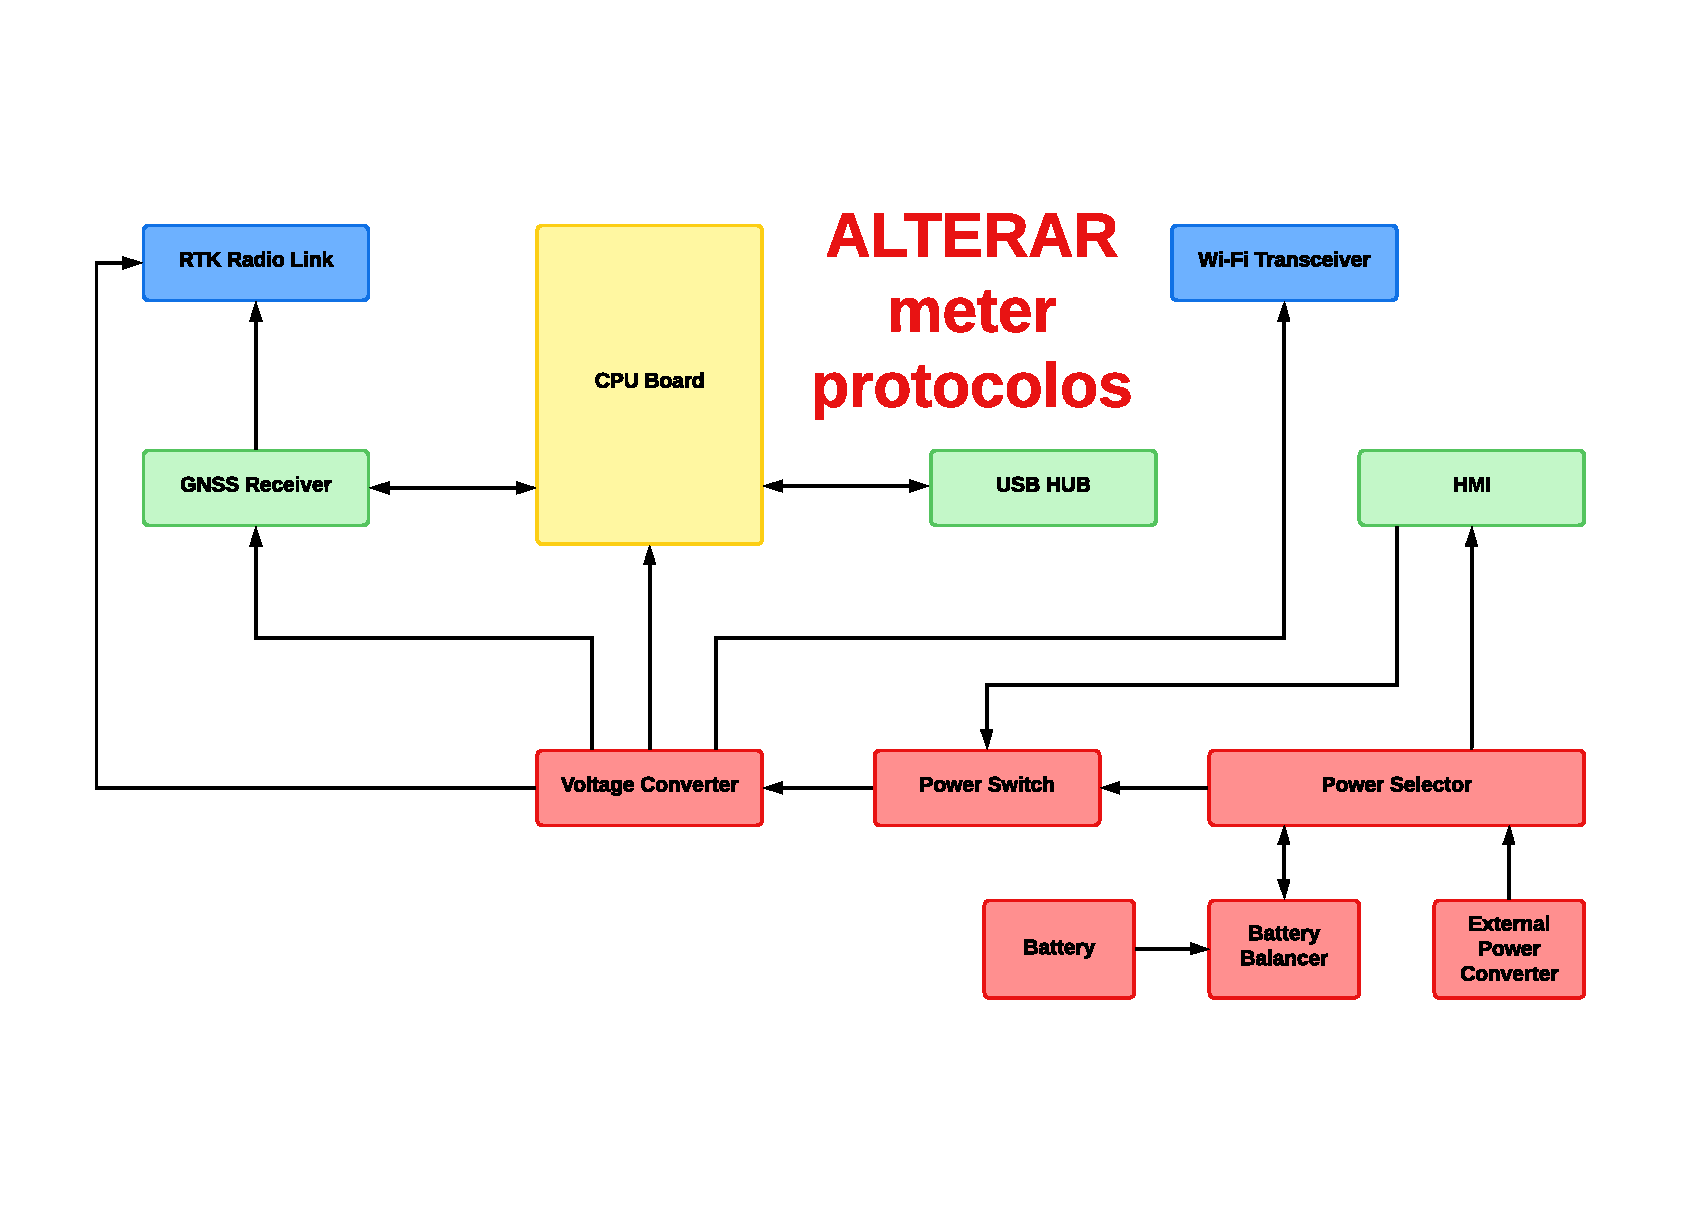
\includegraphics[width=1.0\textwidth]{Chapters/Figures/new_architecture.pdf}
	\caption{beRTK\textsuperscript{\textregistered} Base Station's redesigned block diagram.}
	\label{fig:architecture_new}
\end{figure}

Starting from the control subgroup, the only component to be selected was a single-board computer able to replace the previously used Raspberry Pi 4 Model B; this means the chosen device would have to be able to carry out a pre-determined set of instructions crucial for the operation of the base station. Such requirement is presented in Section~\ref{sec:II_FCT_requirements} -- requirement \textbf{RTKBS.MAIN.FCT.030}, which proposes the use of a single-board computer (SBC).
The set of instructions performed by the original beRTK\textsuperscript{\textregistered} base station is carried out by a Raspberry Pi 4 Model B computer (described in Section~\ref{sec:II_architecture_Control}), therefore, an element with a comparable computational power as this computer would be ideal. The Raspberry Pi Foundation offers a variety of solutions for many project ideas\footnote[7]{The Raspberry Pi Foundation's hardware offers are available at \url{https://www.raspberrypi.com/products/}.}, and since the operations intended for the beRTK\textsuperscript{\textregistered} base station are so well performed by the Raspberry Pi 4 Model B, it would be worth looking through the array of Raspberry Pi products in order to find a good solution. Research leads to the Raspberry Pi Compute Module 4.
This compact module not only has a small form factor when compared with the Raspberry Pi 4 Model B, but it also bears its computational power thanks to the same processor (a Broadcom BCM2711 quad-core Cortex-A72 (ARM v8) 64-bit SoC @ 1.5GHz), which makes it a great option for the system's control unit~\cite{CM4}.

%meter imagem CM4:
\begin{figure}[h]
	\centering
	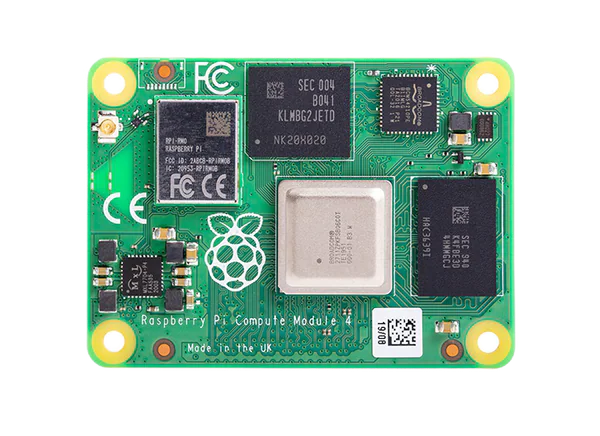
\includegraphics[width=0.5\textwidth]{Chapters/Figures/CM4.png}
	\caption{The Raspberry Pi Compute Module 4 (CM4)~\cite{CM4}.}
	\label{fig:CM4}
\end{figure}

One can choose from thirty-two CM4 variants which differ from each other on RAM and eMMC flash, as well as with or without wireless capabilities. Since this module is intended to be an embedded solution without any of the external ports present in the Raspberry Pi 4 Model B, the relevant ones must be included in the proposed solution, which in this case are USB and HDMI. The CM4 provides all the necessary pins for the implementation of two HDMI connectors on its carrier board (in this case the base station); however, when it comes to using its USB interface, the user must add a USB hub, since only two USB data pins are provided, along with a USB On-The-Go (OTG) pin. The latter is used in order to define the CM4 as either a host or a slave~\cite{CM4}.

%meter imagem do HUB usb: LAN9514

In order to enable such data transfers, the base station would need a component designed to allow the setup of both upstream and downstream USB ports. The Raspberry Pi 3 Model B uses a chip known as LAN9514, which is a four-port USB hub with ethernet functionality. Since this chip has the needed characteristics for the setup of the CM4's USB interface, it was chosen as the main module concerning USB data transfer.

The datasheet for LAN9514 details the chip as a 10/100 ethernet controller, as well as a USB 2.0 hub with four downstream ports and one upstream port, and targets it for desktop computers and embedded systems, among other uses~\cite{LAN9514}. The LAN9514 also fits the Peripherals subgroup, along with the ZED-F9P GNSS receiver and the HMI, the latter of which bridges the user-device gap via a simple on/off button, LED indicators for both battery status and power source indication and a single connector intended for an external power source, satisfying requirement \textbf{RTKBS.MAIN.PWS.050}, as well as all the requirements defined in Section~\ref{sec:II_HMI_requirements}.

The secondary power arrangement in the original beRTK\textsuperscript{\textregistered} design featured two external batteries that would feed the entire system once the mains power supply was disconnected. This form of supply poses considerable disadvantages when it comes to a continuous operation, due to the impractical need of removing the batteries in order to charge them. In the system's power supply subgroup, this was the main improvement to be made following the requirements defined in Section~\ref{sec:II_PWS_requirements}. For that, the base station's enclosure sould count on an internal battery (requirement \textbf{RTKBS.MAIN.PWS.020}) that must not be removed (such battery could be comprised of either a single or multi-cell arrangement) on which the system could rely once the external power supply was disconnected. This idea would help meet requirement \textbf{RTKBS.MAIN.MEC.030}, proposing however a new issue, namely, the charging of the internal battery arrangement.
%meter LINK PARA CADA REQUIREMENT

Referring to requirements \textbf{RTKBS.MAIN.FCT.020} and \textbf{RTKBS.MAIN.FCT.040}, which correspond to the GNSS receiver (ZED-F9P) and the Wi-Fi transceiver (Digi XBee\textsuperscript{\textregistered} 3), respectively, there are no changes in such elements for the new beRTK\textsuperscript{\textregistered}'s proposed solution.

Keeping all this information in mind, 
The original beRTK\textsuperscript{\textregistered}'s design featured a prioritized PowerPath\textsuperscript{\texttrademark} controller, as mentioned in Section~\ref{sec:II_architecture_PowerSupply}. As per Analog Devices, a PowerPath\textsuperscript{\texttrademark} controller is a device able to control the flow of power through a system, while also selecting its power source.


An ideal approach would be to find an IC able to 

With all this in mind, a wise starting point for the research of a power selector able to provide a smooth transistion between an external and internal supply would be from Analog Devices' power management ICs; specifically, from the battery charger ICs. The most well-suited IC found was LTC4012, which is a high efficiency, multi-chemistry battery charger with PowerPath\textsuperscript{\texttrademark} control~\cite{LTC4012}. This battery charger is able to

\section{Circuit Design}\label{32_Circuit}

\section{PCB Layout Design}\label{33_PCBlayout}

